\section{Photon statistics}\label{sec:photon-statistics}
Intensity fluctuations can be regarded as fluctuations in the number of photons emitted by a source. Because of that, we can use \textbf{photon number distribution function} in order to classify light. In particular we have three type of photon statistics:

\begin{enumerate}
    \item \textbf{Super-Poissonian}: 
    \begin{itemize}
        \item Thermal light, incoherent/ partially coherent light 
        \item $I(t)$ is time dependent
        \item $\Delta n > \sqrt{\overline{n}}$
    \end{itemize}
    \item \textbf{Poissonian}: 
    \begin{itemize}
        \item Perfectly coherent light 
        \item $I(t)$ is constant
        \item $\Delta n = \sqrt{\overline{n}}$
    \end{itemize}
    \item \textbf{Sub-Poissonian}: 
    \begin{itemize}
        \item Not-classical light 
        \item $I(t)$ is constant
        \item $\Delta n <\sqrt{\overline{n}}$
    \end{itemize}
\end{enumerate}

\begin{table}[H]
\label{tab:photon-statistics}
\centering
\begin{tabular}{|c|c|c|c|}
\hline
\textbf{Statistics} & \textbf{Type of light} & \textbf{Intensity $I(t)$} & \textbf{Fluctuations} \\
\hline
Super-Poissonian & Thermal / incoherent (partially coherent) & Time dependent & $\Delta n > \sqrt{\overline{n}}$ \\
\hline
Poissonian & Perfectly coherent & Constant & $\Delta n \approx \sqrt{\overline{n}}$ \\
\hline
Sub-Poissonian & Non-classical light & Constant & $\Delta n < \sqrt{\overline{n}}$ \\
\hline
\end{tabular}

The \hl{first two types of statistics are consistent with classical theory of light}, while the third one leads to quantum description. This happens because light is very sensitive to losses and we need an efficient detective system that it has been observed only recently.

\subsection{Poissonian photon statistics}\label{subsec:poissonian-light}
Suppose we have a \textbf{coherent light} beam:
\[
E(x,t) = E_0 \cdot \cos(kx-\omega_0 t + \phi),
\]

where $E_0$ and $\phi$ are fixed, and $k = \frac{\omega_0}{c}$.\\
The intensity is proportional to $|E(t)|^2$, where $E(t)$ is averaged over an optical cycle. In this case, the intensity is constant in time, which implies that the \textit{average} photon flux is constant.

\question{Is the stream of photons emitted at regular time intervals?}{%
The answer is \textbf{NO}. Even though the intensity is constant, the arrival times of photons exhibit statistical fluctuations on short time scales. A coherent light beam is therefore characterized by \textbf{Poissonian photon statistics}.
}

\textbf{Derivation:}
\begin{proof}
Assume a light beam with constant optical power $P$ and photon flux $\Phi$. Let $\overline{n}$ be the average number of photons within a beam segment of length $L$:
\[
\Phi = \frac{P}{\hbar \omega}, \qquad \overline{n} = \Phi \cdot \frac{L}{c}.
\]

Divide the segment $L$ into $N$ sub-intervals, with $N$ large enough that the probability of finding one photon in a given interval is
\[
p = \frac{\overline{n}}{N},
\]

while the probability of finding more than one photon in the same interval is negligible. The probability of finding $n$ intervals containing one photon and $N-n$ empty intervals is given by the binomial distribution:
\[
\begin{split}
P(n) &= \frac{N!}{n!(N-n)!}\cdot p^n\cdot (1-p)^{N-n} \\
&= \frac{N!}{n!(N-n)!}\cdot \left(\frac{\overline{n}}{N}\right)^n \cdot \left(1-\frac{\overline{n}}{N}\right)^{N-n}.
\end{split}
\]

In the limit $N \to \infty$, this expression converges to the \textbf{Poisson distribution}:
\begin{equation}\label{eqn:7-poisson-distribution}
P(n) = \frac{1}{n!}\cdot (\overline{n})^n\cdot e^{-\overline{n}}, \qquad n=0,1,2,\dots
\end{equation}

\end{proof}

Notice that:
\begin{itemize}
    \item The distribution peaks around $\overline{n}$;
    \item The variance is
    \[
    (\Delta n)^2 \coloneqq \sigma^2 = \sum_{n=0}^{\infty} (n-\overline{n})^2 P(n) = \overline{n};
    \]
    \item Standard deviation is
    \[
    \Delta n \coloneqq \sigma = \sqrt{\overline{n}},
    \]
    which shows that fluctuations increase with the mean photon number, while the relative fluctuations decrease as $1/\sqrt{\overline{n}}$.
\end{itemize}
\subsection{Super Poissonian light}\label{subsec:7-super-poissonian-light}

\subsubsection{Black body behavior}\label{subsubsec:7-black-body-behavior}

A \textbf{black body} can be modeled as an \textbf{enclosed cavity at temperature $T$} filled with electromagnetic radiation. In this case, the field consists of a continuous spectrum of oscillating modes with \textbf{energy density} $\rho(\omega,T)$, where $\omega$ is the angular frequency of a given mode. Each mode behaves as a quantized harmonic oscillator with energy:
\begin{equation}\label{eqn:7-energy-of-a-mode}
E_n=\hbar\omega\left(n+\frac{1}{2}\right).
\end{equation}

This leads to the Planck distribution:
\[
\rho(\omega,T)\ \d\omega = \frac{\hbar \omega^3}{\pi^2 c^3}\  
\frac{1}{e^{\beta \hbar \omega}-1}\ \d\omega.
\]

According to Boltzmann statistics, the probability that there are $n$ photons in a single mode of angular frequency $\omega$ is

\begin{equation}
P_{\omega}(n) = 
\frac{e^{-\beta E_n}}{\sum_{n=0}^{\infty} e^{-\beta E_n}}= 
\frac{e^{-\beta \cdot \hbar \omega \cdot n}}
{\sum_{n=0}^{\infty} e^{-\beta \cdot \hbar \omega \cdot n}}
\end{equation}

which is something in the form of $\frac{x^n}{\sum x^n}$, where:
\begin{equation}
\sum x^n = \frac{1}{1-x}, \qquad x=e^{-\beta\hbar\omega}
\end{equation}

so that:
\begin{equation}
P_{\omega}(n) = 
e^{-\beta\cdot \hbar \omega \cdot n}\  
\left(1-e^{-\beta\cdot \hbar \omega}\right),
\end{equation}

\begin{figure}[H]
    \centering
    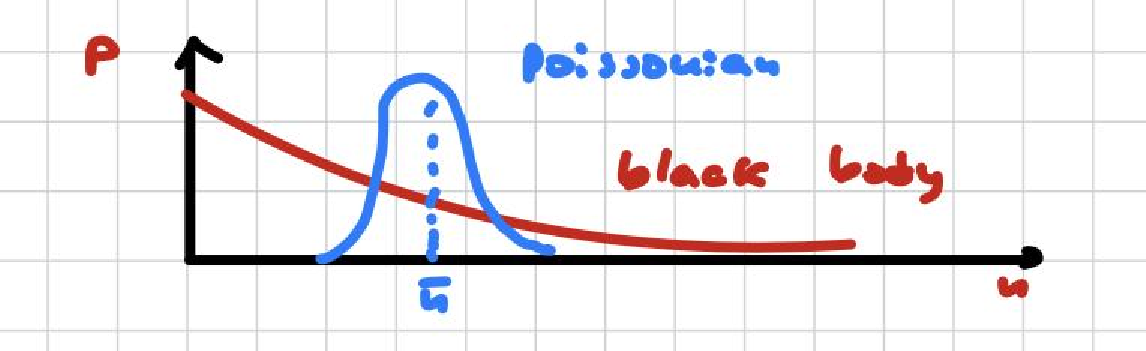
\includegraphics[width=0.8\linewidth]{images_in_pdf/7-/Grafico_28.pdf}
\end{figure}

Observe that the maximum of the distribution is at $n=0$ and that the probability decreases exponentially with $n$. From this expression one obtains the mean photon number and the \textbf{Bose-Einstein distribution}:
\[
P_{\omega}(n)= \frac{1}{\overline{n}+1}\cdot \left(\frac{\overline{n}}{\overline{n}+1}\right)^n,
\qquad
\overline{n}=\frac{1}{e^{\beta\hbar\omega}-1}.
\]

The variance is
\[
\sigma^2 = (\Delta n)^2 = \overline{n}+\overline{n}^2,
\]

hence:
\begin{equation}\label{eqn:7-super-poissonian-variance}
(\Delta n)^2_{\text{Bose}} > (\Delta n)^2_{\text{Poissonian}}.
\end{equation}

The fluctuations are therefore larger than in the Poissonian case, which means that the photon-number distribution of thermal light is broader than that of coherent light. Thermal light is thus \textbf{super-Poissonian}.

\calloutwarn{%
\textbf{Be aware!} The Bose-Einstein distribution applies to a single mode, whereas a black body contains a continuum of modes. If many independent modes are collected in the same detection time, the bunching contribution is reduced. In a multimode measurement one often writes
\[
(\Delta n)^2 = \overline{n}+\frac{\overline{n}^2}{M},
\]
where $M$ is the number of independent modes contributing to the detected signal; in the limit $M\to\infty$, the excess fluctuation term is suppressed and the statistics can approach Poissonian behavior. In a real experiment, observing a strictly single-mode thermal field is difficult, because mode averaging and interference effects tend to wash out part of the bunching signal.
}

\subsubsection{Discharge lamp behavior}\label{subsubsec:7-discharge-lamp-behavior}

Suppose we have a discharge lamp with a single spectral line. Such a source is a chaotic light source, meaning that it exhibits classical intensity fluctuations on a timescale set by the coherence time $\tau_c$. The fluctuations in the photon number, when the flux is measured over a detection time $T$, are given by
\begin{equation}\label{eqn:7-fluctuations-discharge-lamp}
(\Delta n)^2 = \langle W(T)\rangle + \langle \delta W(T)^2\rangle.
\end{equation}

\hl{The first term comes from \textbf{Poissonian shot noise}, which reflects the particle nature of light, while the second term represents classical power fluctuations}.

Here:
\begin{itemize}
    \item $W(T)$ is the count rate within a detection time $T$:
    \[
    W(T) = \int_t^{t+T} \eta \, \Phi(t')\,dt',
    \]
    \item $\eta$ is the detection efficiency,
    \item $\Phi = \frac{P}{\hbar\omega}$ is the instantaneous photon flux,
    \item $\delta W(T) = W(T)-\langle W(T)\rangle$ denotes the classical fluctuation of the detected signal.
\end{itemize}

Notice that if $\Phi$ is constant, then
\[
\langle \delta W(T)^2\rangle = 0
\]

and one recovers the Poissonian result
\[
(\Delta n)^2 = \overline{n}.
\]

In our case, however, $\Phi \neq \text{constant}$ and \textbf{two different regimes} can be identified:

\begin{enumerate}
    \item \emph{The intensity fluctuations are relevant when}
    \begin{equation}\label{eqn:7-fluctuations-relevant}
    T \leq \tau_c \implies \langle \delta W(T)^2\rangle \neq 0.
    \end{equation}

    In this regime, the \hl{detection time is short enough that the detector can resolve the temporal fluctuations of the light field}. Since the phase and intensity remain correlated over a time of order $\tau_c$, the measured signal reflects not only the Poissonian shot noise (due to the particle nature of light), but also the classical intensity fluctuations of the source. Physically, this corresponds to the fact that thermal light exhibits photon bunching, so photons tend to arrive in correlated groups rather than independently.
    \item \emph{The Poissonian behavior is approached when}
    \begin{equation}\label{eqn:7-poissonian-limit}
    T > \tau_c \implies \Phi \approx \text{constant}.
    \end{equation}

    In this case, the detector integrates the signal over many independent coherence intervals. As a result, the rapid phase and intensity fluctuations average out, and the contribution of classical power fluctuations is strongly reduced:
    \[
    \langle \delta W(T)^2\rangle \to 0.
    \]
    The measured statistics therefore approaches the Poissonian limit, where fluctuations are dominated by shot noise. Physically, \hl{this does not mean that the light itself becomes Poissonian, but rather that the measurement process averages over the fluctuations, making the detected signal appear more regular}.
\end{enumerate}
\subsection{Sub-Poissonian light}
By definition $\Delta n < \sqrt{\overline{n}}$, it has not a classical equivalent and it is a clear signature of quantum nature of light.

Suppose to have a light beam where every time interval between the photons is the same $\Delta x = c \Delta t$. In a time $T$ the photocount will be:
\begin{equation}\label{eqn:7-sub-poissonian-photocounts}
N = \mathrm{int} 
\biggr(
    \eta \cdot \frac{T}{\Delta t}
\biggr)
\end{equation}
\begin{figure}[H]
    \centering
    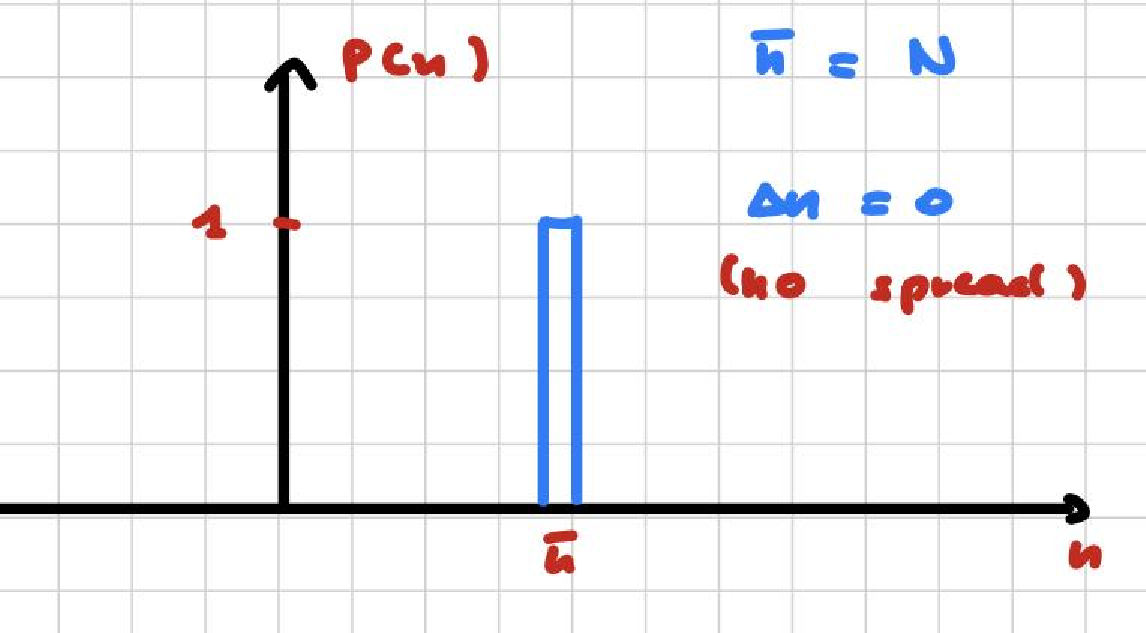
\includegraphics[width=0.8\linewidth]{images_in_pdf/7-/Grafico_29.pdf}
\end{figure}

This kind of photon stream is called \textbf{Photon Number states}. Observe that the time intervals $\Delta t$ are not exactly the same, but more \say{regular} than the random intervals pertaining to beams having poissonian statistics.

\calloutwarn{%
Sub-poissonian instead is very fragile and for this reason we need to avoid optical losses and have high-efficiency detectors.

The main factors that degrade photon statistics are:
\begin{itemize}
    \item Inefficient collection of light emitted by source;
    \item Absorption/scattering/reflection from optical components;
    \item Imperfect quantum detection.
\end{itemize}
}

\hl{This leads us to study photodetection}.

\subsubsection{Photodetection}\label{subsubsec:7-photodetection}

\question{How are the electric field and light intensity converted into an experimental signal?}{%
Photodetectors operate by absorbing a portion of the incoming light beam and converting its energy into a measurable electrical signal.}

For example, consider a red laser with wavelength $\lambda = \qty{633}{\nano\meter}$ and a very low power $P \approx \qty{1}{\nano\watt}$; the \textbf{photon flux} impinging on the detector is still huge:
\begin{equation}\label{eqn:7-photon-flux-example}
\Phi = \frac{IA}{\hbar \omega} = \frac{P}{\hbar \omega} \approx 3\cdot 10^9 \ \text{photons/s}.
\end{equation}

This high photon flux motivates the use of devices capable of counting individual photons within a given time interval $\Delta t$: \textbf{photon counters}.

We can define:

\begin{itemize}
\item  the \textbf{quantum efficiency} of the detector, or probability that an incident photon produces a photocount:
\begin{equation}\label{eqn:7-quantum-efficiency}
\eta = \frac{\text{Number of photocounts}}{\text{Number of incident photons}};
\end{equation}

\item  the \textbf{average number of counts} recorded during a time interval $T$: 
\begin{equation}\label{eqn:7-average-counts}
M(T) = \eta \cdot \Phi \cdot T = \eta \cdot \frac{P}{\hbar \omega} \cdot T;
\end{equation}

\item the corresponding \textbf{average count rate}:
\begin{equation}\label{eqn:7-average-count-rate}
R = \frac{M(T)}{T} = \eta \cdot \frac{P}{\hbar \omega} \quad [\text{counts/s}].
\end{equation}

\end{itemize}

\calloutwarn{If the detector has a \textbf{dead time}, which is a recovery period after each detection event, this limits the maximum count rate. For instance, a dead time of \qty{1}{\nano\second} determines a \emph{maximum rate} of $R \approx 10^9$ counts/s.}

It is also important to observe that $R$ and $\Phi$ are \textbf{average quantities}, while the actual photon flux exhibits statistical fluctuations due to the discrete nature of light. \hl{These fluctuations of the measured count rate $R$ can be used to study the photon statistics of the light beam.}

However, in addition to the intrinsic photon statistics of the light, \textbf{the detector itself introduces fluctuations because the detection process is probabilistic:}
\begin{itemize}
    \item Each photon is registered with probability $\eta$, so the photocounts follow a \textbf{Bernoulli process} for each incident photon.
    \item Additional sources of fluctuation include dark counts, electronic noise, dead time effects, and imperfect detection efficiency.
\end{itemize}
As a result, the observed photocounts reflect both the \hl{statistical properties of the light beam} and the \hl{stochastic nature of the detection process}. Therefore, when analyzing photon statistics, it is essential to distinguish between fluctuations due to the light source itself and those introduced by the detector.
\subsubsection{Semiclassical theory}
In order to study photo-counting detectors, we start with the photomultiplier.
\begin{figure}[H]
    \centering
    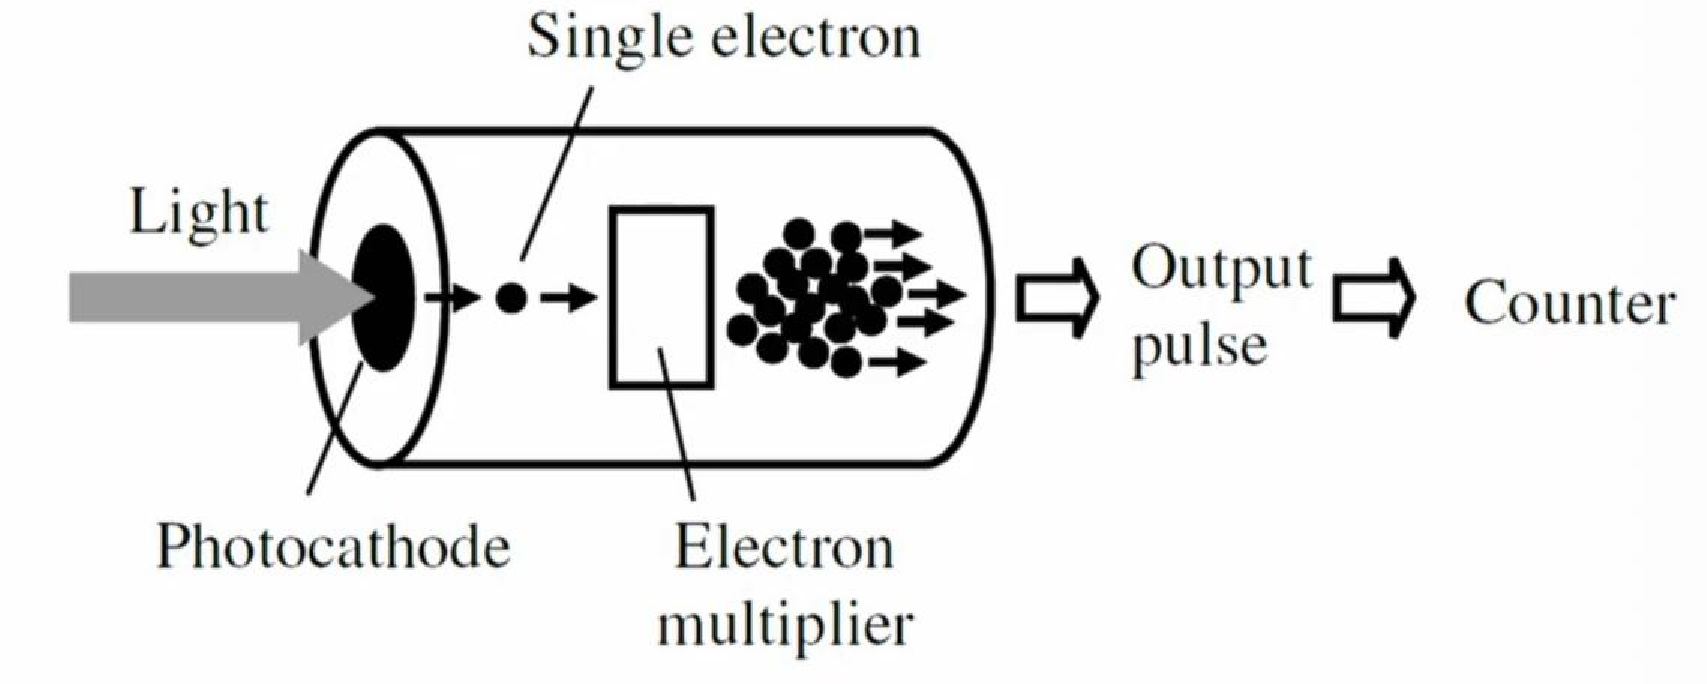
\includegraphics[width=0.8\linewidth]{images_in_pdf/7-/Grafico_30.pdf}
\end{figure}

Suppose that a light beam impinges on a photocathode, so that a single electron is emitted by the \textbf{photoelectric effect} and then amplified by an electron multiplier. This process gives rise to an output pulse and, consequently, to a count.

\hl{In the semiclassical framework, atoms and the detector are treated quantum mechanically, while the electromagnetic field is treated classically}. The number of photocounts produced in an integration time $T$ is therefore a measure of the optical intensity. We consider a large number of successive measurements, each performed over the same integration time, in order to build the probability distribution $P_n(T)$ for observing $n$ photocounts during the interval $T$.

The probability that the light causes the emission of one electron, observed as a photocount event between $t$ and $t+dt$, is
\[
p(t)\,dt = \eta\,I(t)\,dt,
\]
where $\eta$ is the detector efficiency and $I(t)$ is the appropriately normalized light intensity. We assume $dt$ to be sufficiently small so that the probability of detecting two electrons in the same interval is negligible.

If we define $P_n(t,\tau)$ as the probability that $n$ photocounts occur in the time interval from $t$ to $t+\tau$, then, after a further short interval $d\tau$, the same $n$ photocounts can be obtained in two ways:

\begin{equation}\label{eqn:7-photon-statistics-derivation}
\begin{split}
    a&.
    \begin{cases}
    a_1.\ n \text{ events} \hspace{0.55cm} &t \to t+\tau\\
    a_2.\ 0 \text{ events}              &t+\tau \to t+\tau+d\tau
    \end{cases}
    \\[1ex]
    b&.
    \begin{cases}
        b_1.\ n-1 \text{ events} &t \to t+\tau\\
        b_2.\ 1 \text{ event}    &t+\tau \to t+\tau+d\tau
    \end{cases}
\end{split}
\end{equation}

hence:
\begin{equation}\label{eqn:7-photon-statistics-probabilities}
\begin{alignedat}{3}
    a&.
    \begin{cases}
        P(a_1) = P_n(t,\tau)\\
        P(a_2) = 1 - p(t+\tau)\,\d\tau
    \end{cases}
    &&\implies\ 
    P(a) = P_n(t,\tau) \left[1 - p(t+\tau)\,\d\tau\right]
    \\[1ex]
    b&.
    \begin{cases}
        P(b_1) = P_{n-1}(t,\tau)\\
        P(b_2) = p(t+\tau)\,\d\tau
    \end{cases}
    &&\implies\ 
    P(b) = P_{n-1}(t,\tau)\,p(t+\tau)\,\d\tau
\end{alignedat}
\end{equation}

The total probability is then
\begin{equation}\label{eqn:7-photon-statistics-total-probability}
\begin{split}
    P_n(t,\tau+d\tau) &= P_n(t,\tau)\,[1-p(t+\tau)\,d\tau] + P_{n-1}(t,\tau)\,p(t+\tau)\,d\tau\\
    &= P_n(t,\tau) - \eta I(t+\tau)P_n(t,\tau)\,d\tau + \eta I(t+\tau)P_{n-1}(t,\tau)\,d\tau,
\end{split}
\end{equation}

which gives
\[
\frac{dP_n(t,\tau)}{d\tau}=\eta\,I(t+\tau)\,[P_{n-1}(t,\tau)-P_n(t,\tau)].
\]

For $n=0$, the term $P_{-1}$ vanishes, so
\[
\frac{dP_0(t,\tau)}{d\tau}=-\eta\,I(t+\tau)\,P_0(t,\tau).
\]

Since there are no photocounts in a zero-time interval, the boundary conditions are
\[
P_0(t,0)=1, \qquad P_n(t,0)=0 \quad \forall\, n\ge 1.
\]

Using these boundary conditions and solving recursively, we obtain the \textbf{Mandel formula}
\[
P_n(t,T)=\frac{1}{n!}\left[\eta \int_t^{t+T} I(t')\,dt'\right]^n
\exp\!\left[-\eta \int_t^{t+T} I(t')\,dt'\right].
\]

If we define the average intensity over the integration time as
\[
I(t,T)=\frac{1}{T}\int_t^{t+T} I(t')\,dt',
\]

then the formula can be written as
\[
P_n(t,T)=\frac{1}{n!}\,[\eta\,I(t,T)\,T]^n\,e^{-\eta\,I(t,T)\,T},
\qquad
P_0(t,T)=e^{-\eta\,I(t,T)\,T}.
\]

It can also be shown that
\[
\overline{n}=\sum_n n\,P_n(t,T)=\eta\,\langle I(t,T)\rangle\,T.
\]

From here, we have two scenarios:

\textbf{1} Classical stable wave:
\[
\langle I(t,T)\rangle=\text{constant} \implies \eta\,\langle I\rangle = C.
\]

We can calculate $P_n$ in the limit $d\tau \to 0$:
\[
\frac{dP_n}{d\tau}=C\,[P_{n-1}-P_n] \implies \frac{dP_n}{d\tau}+C\,P_n=C\,P_{n-1}.
\]

If $n=0$, then $P_{n-1}=0$, and therefore
\[
\begin{cases}
\frac{dP_0}{d\tau}=-C\,P_0\\
P_0(0)=1
\end{cases}
\implies P_0(T)=e^{-CT}.
\]

For $n\ge 1$, using the integrating factor $e^{CT}$, we obtain
\[
\frac{d}{d\tau}\!\left[P_n(\tau)e^{C\tau}\right]=C\,P_{n-1}(\tau)e^{C\tau},
\]

so that
\[
P_n(T)=e^{-CT}\int_0^T d\tau\, C\,e^{C\tau}\,P_{n-1}(\tau).
\]

We can solve this recursively:
\[\begin{split}
    P_1(T) &= e^{-CT}\int_0^T d\tau\, C\,e^{C\tau}\,P_0(\tau)
    = e^{-CT}\int_0^T d\tau\, C
    = e^{-CT}\,CT,\\
    P_2(T) &= e^{-CT}\int_0^T d\tau\, C\,e^{C\tau}\,P_1(\tau)
    = e^{-CT}\,\frac{(CT)^2}{2},\\
    P_n(T) &= e^{-CT}\,\frac{(CT)^n}{n!}.
\end{split}\]

Since
\[
\overline{n}=\eta\,\langle I\rangle\,T=CT,
\]

we finally obtain
\[
P_n(T)=\frac{\overline{n}^{\,n}}{n!}\,e^{-\overline{n}}.
\]

\calloutinfo{Thus, we recover the Poisson distribution, which means that the photocount statistics are the same as those of particle emission in radioactive decay.

A measurement of the continuous time-dependent intensity of a classical wave by means of a photomultiplier produces discrete photocounts with a well-defined distribution.}

Observe that we obtain Poissonian statistics without invoking photons explicitly, we only assume that
\begin{itemize}
    \item emission of photoelectrons is probabilistic;
    \item light energy is absorbed in discrete detection events.
\end{itemize}
However, \textbf{the photocount statistics do not, by themselves, reveal the full quantum nature of light. A classical field with constant intensity leads to Poissonian counting, while sub-Poissonian statistics require a more general quantum theory of the electromagnetic field.}
\subsubsection{Quantum theory of photodetection}
Assume that we have:
\begin{itemize}
    \item The variance of the photocount number is
    \[
    (\Delta N)^2 = \eta^2 (\Delta n)^2 + \eta(1-\eta)\,\overline{n},
    \]
    The first term in the variance,
\[
\eta^2 (\Delta n)^2,
\]
represents the fluctuations already present in the incoming light, reduced by the finite efficiency of the detector. The second term,
\[
\eta(1-\eta)\,\overline{n},
\]
is the additional noise introduced by the detection process itself, due to the random loss of photons. \\
    \item The quantum efficiency is
    \[
    \eta = \frac{\overline{N}}{\overline{n}},
    \]
    where $\overline{N}$ is the average photocount number and $\overline{n}$ is the mean photon number impinging on the detector.
\end{itemize}
We can have:
\begin{enumerate}
    \item If $\eta = 1$, then $\Delta N = \Delta n$, so the photon counts faithfully reproduce the fluctuations of the incident photon stream.\\
    \item If $(\Delta n)^2 = \overline{n}$, i.e. the incident light has Poissonian statistics, then
    \[
    (\Delta N)^2 = \eta \overline{n} = \overline{N} \qquad \forall\, \eta,
    \]
    which means that the photocount fluctuations remain Poissonian.
\end{enumerate}
\textbf{A detector with efficiency $\eta$ can be modeled as a perfect detector preceded by a beam splitter of transmittance $\eta$}, which randomly selects which photons are actually detected, independently of the original state of light. In this sense, the detection process is equivalent to a binomial thinning of the incident photon number distribution. \\\\
\textbf{If $\eta \ll 1$, the detected photocount stream becomes strongly randomized and tends toward Poissonian statistics}, even if the original light state had reduced fluctuations. For this reason, \textbf{low quantum efficiency tends to mask sub-Poissonian behavior} and makes it difficult to observe nonclassical light experimentally. \\
In practice, it is difficult to realize detectors with very high quantum efficiency ($\eta > 50\%$), and this is one of the reasons why observing sub-Poissonian statistics is experimentally challenging.
\subsubsection{Quantum noises}
Let us start with \textbf{photodiodes}. Consider a $p$-$n$ junction under reverse bias. When external light impinges on the junction, it generates electron-hole pairs, which are then separated by the electric field and collected at the contacts. This process gives rise to a \textbf{photocurrent} $i$: 
\begin{figure}[H]
    \centering
    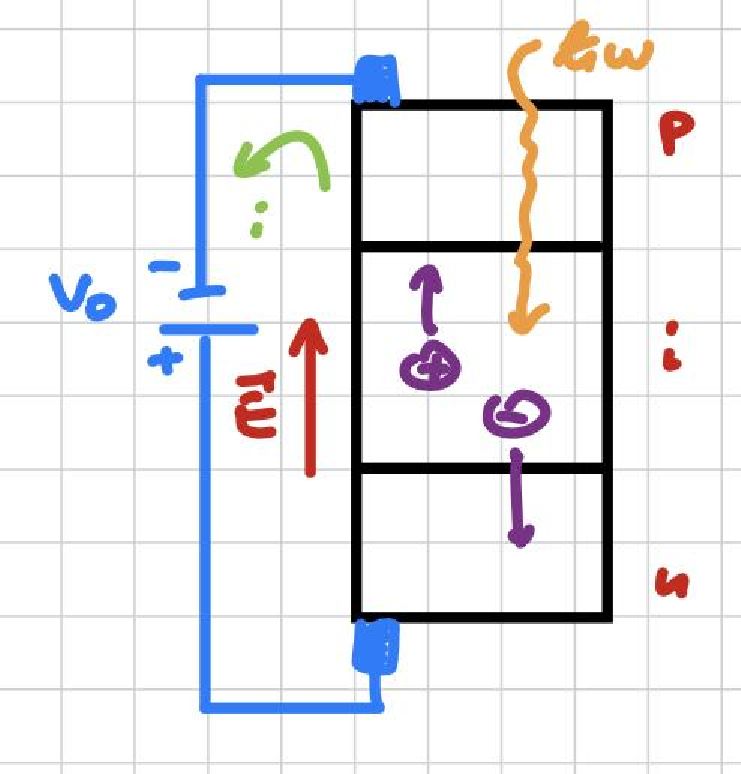
\includegraphics[width=0.5\linewidth]{images_in_pdf/7-/Grafico_31.pdf}
\end{figure}

The \textbf{photodiode responsivity} can be defined as
\[
i = \eta\,|e|\,\Phi = \eta\,|e|\,\frac{P}{\hbar\omega}
\qquad \Rightarrow \qquad
\frac{i}{P} = \eta\,\frac{|e|}{\hbar\omega}
\hspace{0.5cm}\left[\frac{A}{W}\right],
\]
where $\Phi$ is the photon flux, $P$ is the optical power, and $\eta$ is the quantum efficiency. More precisely, the responsivity depends on wavelength through $\hbar\omega = hc/\lambda$, so that
\[
\frac{i}{P}=\eta\,\frac{|e|\lambda}{hc}.
\]
We now connect the photodiode to a load resistor and measure the output voltage $V(t)$ using an amplifier and filtering the signal. The photocurrent produces
\[
V(t)=i(t)\,R_L.
\]
\begin{figure}[H]
    \centering
    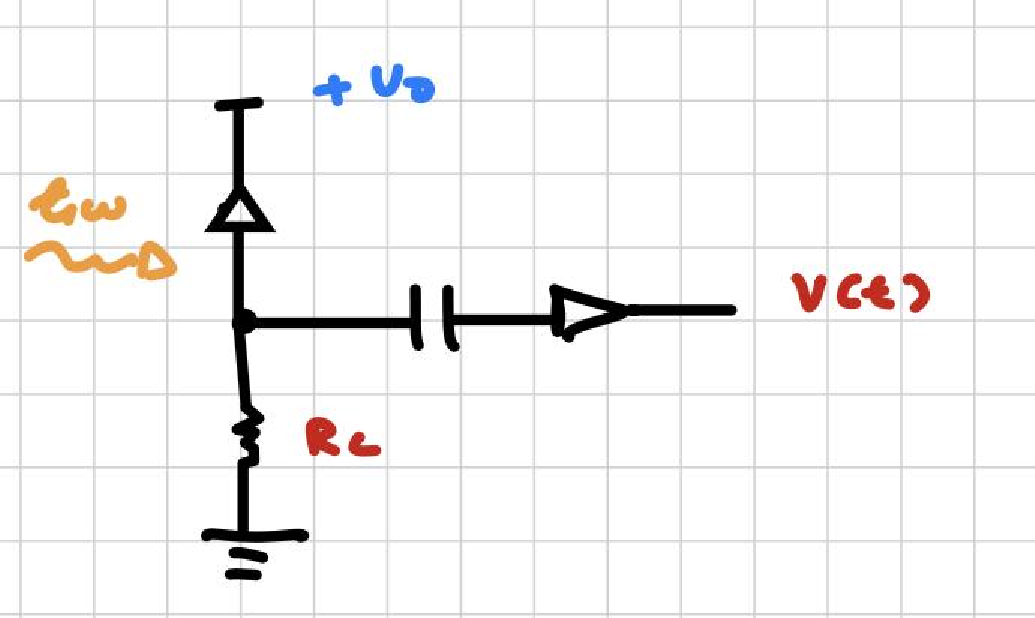
\includegraphics[width=0.8\linewidth]{images_in_pdf/7-/Grafico_32.pdf}
\end{figure}

The measured current can be decomposed into a mean value and a fluctuation:
\[
i(t)=\langle i(t)\rangle+\Delta i(t).
\]
\begin{figure}[H]
    \centering
    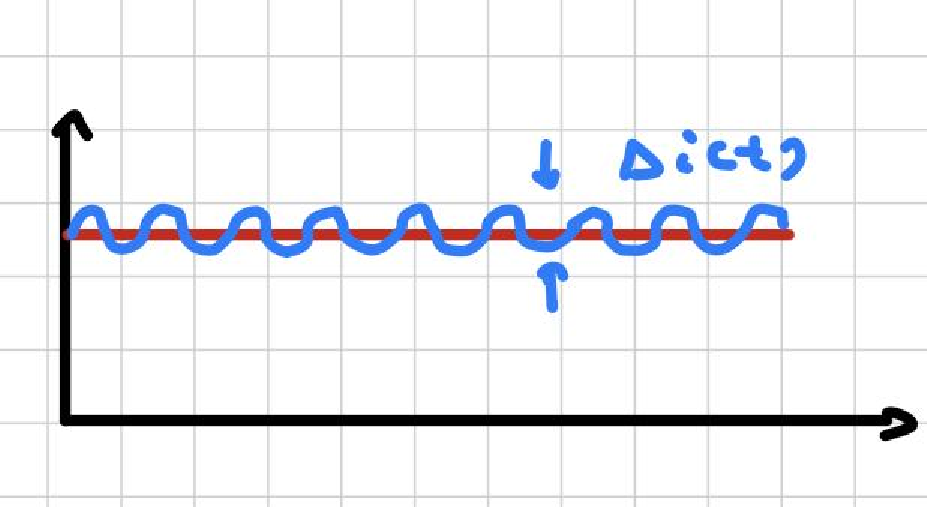
\includegraphics[width=0.8\linewidth]{images_in_pdf/7-/Grafico_33.pdf}
\end{figure}

If the number of detected photons fluctuates, then the photocurrent fluctuates as well, with a detection fidelity set by $\eta$. These fluctuations are precisely the noise:
\[
\langle \Delta i(t)\rangle = 0
\qquad \text{but} \qquad
\langle \Delta i^2(t)\rangle \neq 0.
\]
This is reflected in the electrical power dissipated on the load. In a time-domain description one may write
\[
P_{\text{noise}}(t)=\Delta i^2(t)\,R_L,
\]
while in a frequency-domain treatment it is more precise to consider the noise spectral density of the current or voltage. The decibel scale is
\[
P[\text{dBm}] = 10\log_{10}\!\left(\frac{\text{power}}{1\,\text{mW}}\right).
\]
If we analyze the noise in the frequency domain by Fourier transforming the signal, we can distinguish two different regions:
\begin{figure}[H]
    \centering
    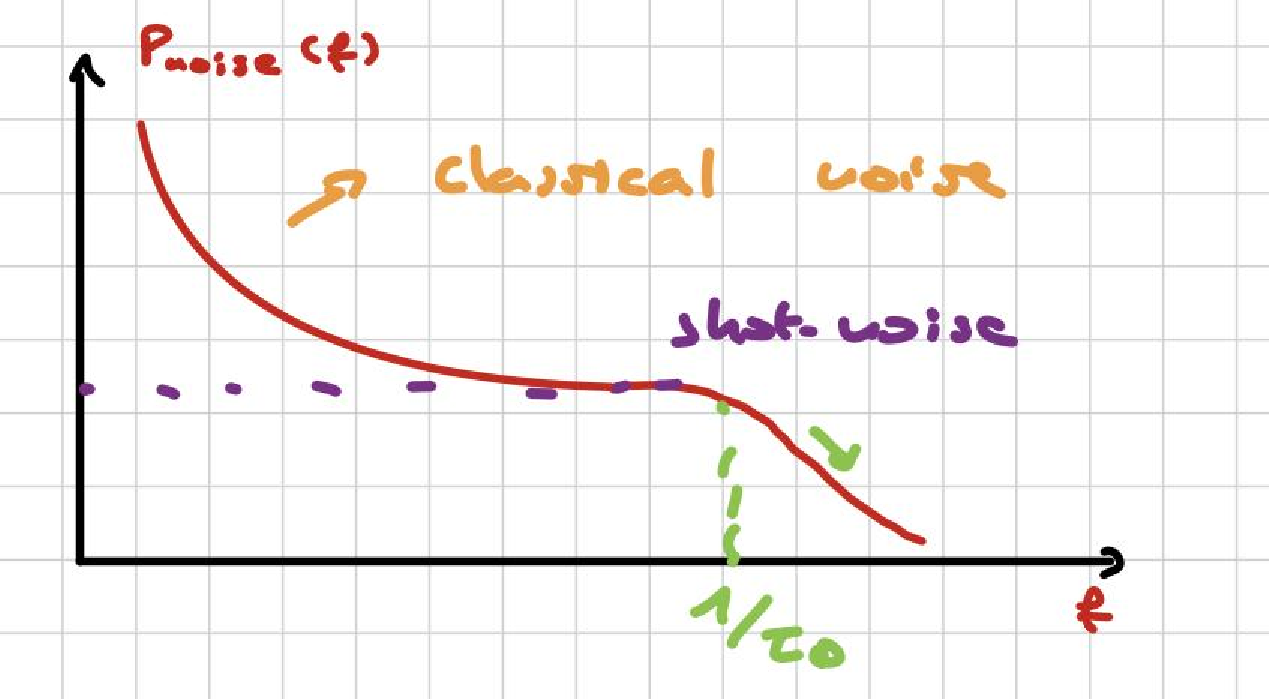
\includegraphics[width=0.8\linewidth]{images_in_pdf/7-/Grafico_34.pdf}
\end{figure}
\newpage
\begin{itemize}
    \item \textbf{Low-frequency limit:} this region is dominated by technical noise, such as fluctuations in the electrical drive current, laser intensity noise, and mechanical vibrations of the optical cavity. In this regime we have \textbf{classical noise}.\\
    \item \textbf{High-frequency limit:} here the technical noise is suppressed and only the fundamental noise associated with photon statistics remains. In this regime we have \textbf{shot noise} or \textbf{quantum noise}.\\
    \item \textbf{High-frequency cut-off:} the noise spectrum eventually decreases to zero because of the finite \textbf{detection response time} $\tau_D$, which limits the bandwidth of the detector.
\end{itemize}
If we consider an ideal coherent light source, we know that the photon statistics are Poissonian. This is reflected in the number of photogenerated charges, for which
\[
(\Delta N)^2 = \langle N\rangle.
\]
Since the photocurrent is proportional to the number of detected charges, the current fluctuations satisfy
\[
(\Delta i)^2 \propto \langle i(t)\rangle,
\]
and therefore
\[
P_{\text{noise}} = (\Delta i)^2\,R_L \propto \langle i(t)\rangle \propto P_{\text{optical}}.
\]
This means that there is a linear relation between noise power and optical power. For a coherent source, this is the hallmark of shot noise:
\begin{figure}[H]
    \centering
    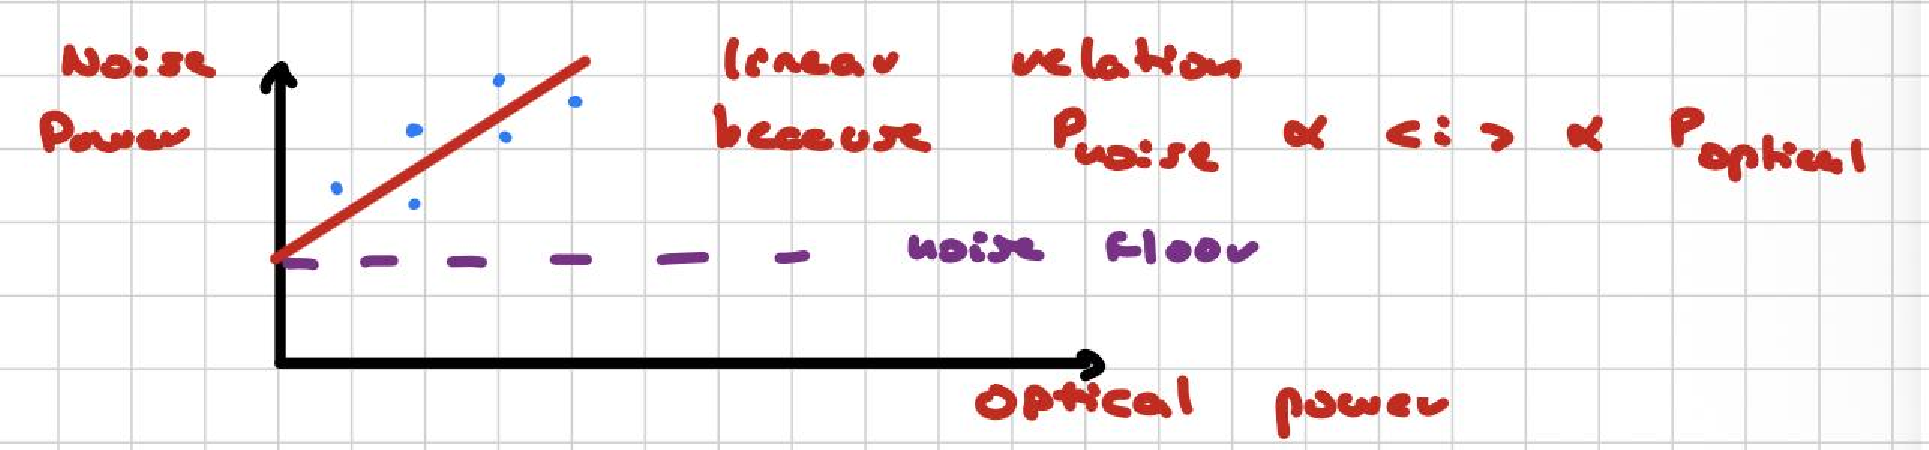
\includegraphics[width=0.8\linewidth]{images_in_pdf/7-/Grafico_35.pdf}
\end{figure}

The \textbf{noise floor} is the background electronic noise of the whole measurement chain, including the amplifier, the load resistor, the cables, and the readout electronics. It is present even in the absence of light and is therefore uncorrelated with the photocurrent. By contrast, \textbf{shot noise} originates from the discrete and random nature of photo-detection events. Even when the average optical intensity is constant, individual photons are detected at random times, and this produces fluctuations in the photocurrent.\\
Shot noise is called \textbf{white} because, within the detector bandwidth, its spectral density is approximately constant as a function of frequency. This does not mean that all physical frequencies contribute equally without limit; rather, it means that the photon-arrival process is essentially delta-correlated on the time scales relevant to the detector. In this sense, shot noise is an intrinsic consequence of the quantized and random character of photo-detection.\\\\
If we want to maximize the \textbf{signal-to-noise ratio} $S/N$, we can modulate the light intensity at a chosen frequency by placing a mechanical chopper in front of the beam. The chopper periodically blocks and transmits the beam, converting a constant (DC) optical signal into a time-dependent (AC) signal at a modulation frequency $f_{\text{mod}}$. 
In this way, the useful signal is shifted from zero frequency to a finite frequency. This does not modify the intrinsic noise sources, but it changes the frequency region in which the measurement is performed. Since technical noise is typically dominant at low frequencies, while shot noise is approximately white within the detector bandwidth, choosing a sufficiently high modulation frequency allows the measurement to be performed in a regime where technical noise is suppressed and the system becomes \textbf{shot-noise limited}.
Therefore, the role of the chopper is not to reduce the noise itself, but to move the signal into a frequency region where the noise is lower and better controlled, improving the overall signal-to-noise ratio.\\\\
Consider now the following setup: a power supply is connected to a laser beam that emits light onto a beam splitter, and one output is reflected onto the detector $D_1$, which is connected to the same power supply.
\begin{figure}[H]
    \centering
    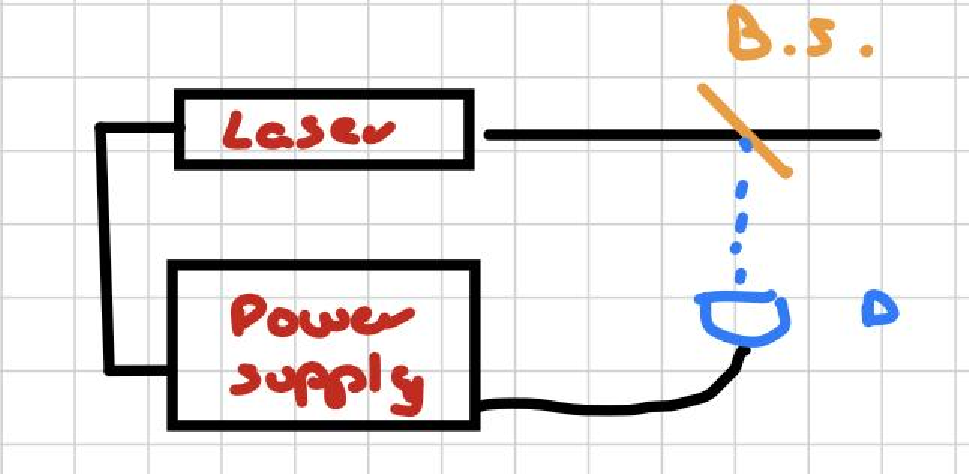
\includegraphics[width=0.8\linewidth]{images_in_pdf/7-/Grafico_36.pdf}
\end{figure}

A small fraction of the laser output is fed back to the power supply. This feedback can reduce classical intensity fluctuations, but it does not modify the fundamental shot-noise contribution.
\begin{figure}[H]
    \centering
    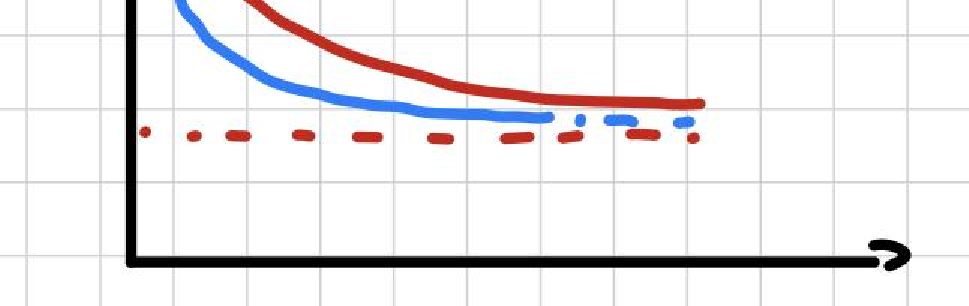
\includegraphics[width=0.8\linewidth]{images_in_pdf/7-/Grafico_37.pdf}
\end{figure}

Suppose instead that a laser beam hits a beam splitter, one part is transmitted to the detector $D_1$ while the other is reflected to detector $D_2$, and the two photocurrents are then combined electronically at a later stage.
\begin{figure}[H]
    \centering
    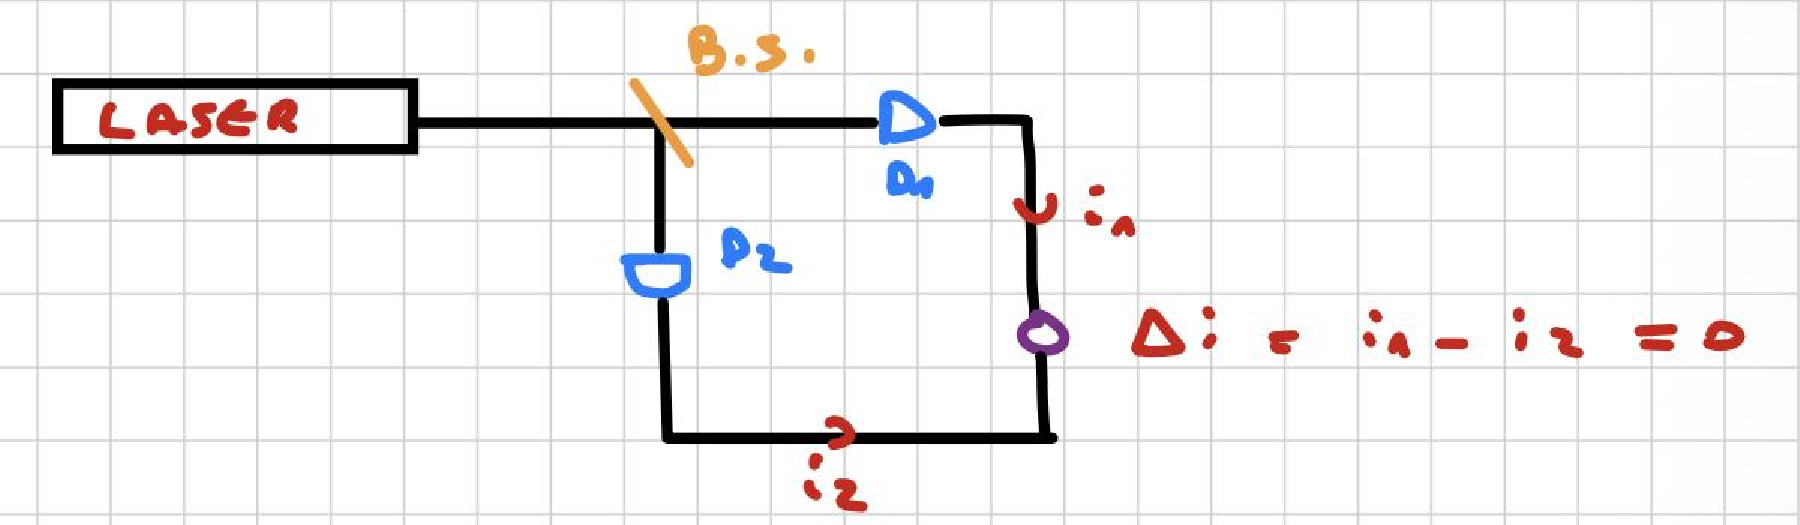
\includegraphics[width=0.8\linewidth]{images_in_pdf/7-/Grafico_38.pdf}
\end{figure}

If there is absorption along one path, the two currents are no longer perfectly equal, so that $\Delta i \neq 0$. This makes it possible to detect very weak variations of light with a better signal-to-noise ratio than with a single detector. This is the idea behind a \textbf{balanced detector}: common-mode technical noise is suppressed by subtraction, while the differential signal survives and can be measured with higher sensitivity.

In this way we can strongly reduce the classical noise component. \textbf{Can we beat the shot-noise limit?} The answer is yes, but only by using nonclassical light sources, such as squeezed states or sub-Poissonian states. In practice, the experimental observation of sub-Poissonian photon statistics also requires detectors with high quantum efficiency $\eta$, because optical losses tend to wash out the nonclassical noise reduction and drive the observed statistics back toward the Poissonian limit.